% !TEX program = XeLaTeX
% !TEX encoding = UTF-8
\documentclass[UTF8,nofonts]{article}
%{ctexart}


%\setCJKmainfont[BoldFont=FandolSong-Bold.otf,ItalicFont=FandolKai-Regular.otf]{FandolSong-Regular.otf}
%\setCJKsansfont[BoldFont=FandolHei-Bold.otf]{FandolHei-Regular.otf}
%\setCJKmonofont{FandolFang-Regular.otf}

\usepackage{url}
\usepackage{cancel}
\usepackage{xspace}
\usepackage{graphicx}
\usepackage{multicol}
\usepackage{multirow}
\usepackage{subfig}
\usepackage{amsmath}
\usepackage{amssymb}
\usepackage[a4paper, width=186mm, top=18mm, bottom=18mm, includeheadfoot]{geometry}
%\usepackage[a4paper, width=140mm, top=18mm, bottom=22mm, includeheadfoot]{geometry}
\usepackage{booktabs}
\usepackage{array}
\usepackage{verbatim}
\usepackage{caption}
\usepackage{natbib}
\usepackage{booktabs}
\usepackage{float}
\usepackage{pdflscape}
\usepackage{mathtools}
\usepackage[usenames, dvipsnames]{xcolor}
\usepackage{afterpage}
\usepackage{pgf}
\usepackage{tikz}
\usepackage{fontspec}
\usepackage{dirtree}
\usepackage[style=american]{csquotes}
\usepackage{amsfonts}
\usepackage{tikz}
\usepackage{tkz-graph}
\usetikzlibrary{arrows,decorations.pathmorphing,automata,positioning,backgrounds,fit,shapes.symbols,chains,intersections}

\newtheorem{definition}{Definition}[section]
\newtheorem{theorem}{Theorem}[section]
\newtheorem{lemma}{Lemma}
\newtheorem{proof}{Proof} [section]


\usepackage[toc, page, title, titletoc, header]{appendix}
\usepackage{marginnote}
\usepackage{tablefootnote}


%\renewcommand\appendixname{附\ 录}
%\renewcommand\appendixpagename{附\ 录}
%\renewcommand\appendixtocname{附\ 录}
\renewcommand\abstractname{Abstract}


\usepackage{perpage} %the perpage package
\MakePerPage{footnote} %the perpage package command

\usetikzlibrary{shapes.geometric}%
\usepackage{color}
%\usepackage[pages=some, placement=top]{background}
\usepackage{eso-pic}
\usepackage[final]{pdfpages}

%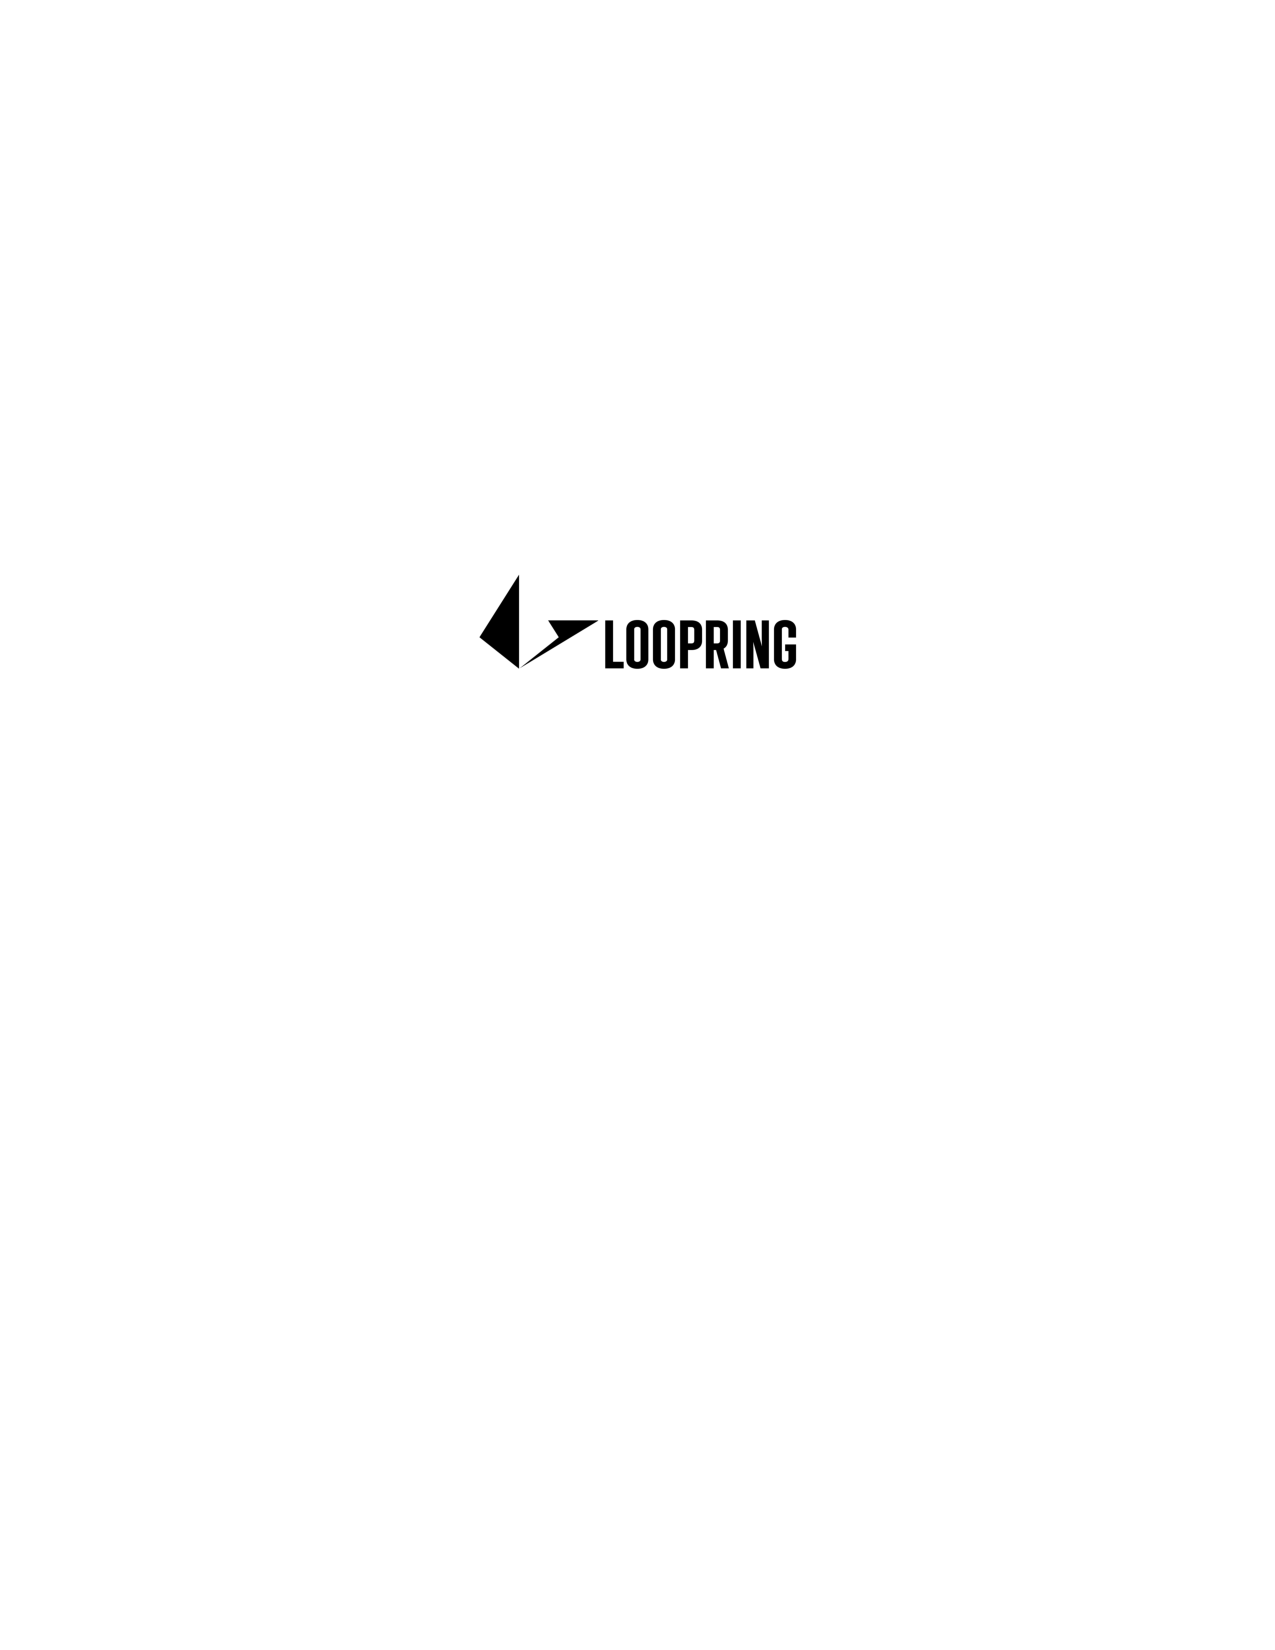
\includepdf[pages=1]{cover}
\hyphenpenalty=750

\title{\textbf{Loopring:}\\\textbf{Un protocole pour marchés d'échange décentralisés}}
\author{
  Daniel Wang\\
  \texttt{daniel@loopring.org}\\
  \and
  	Jay Zhou\\
  	\texttt{jay@loopring.org}\\
  	\and
  	Alex Wang\\
  	\texttt{alex@loopring.org}\\
  	\and
  	Matthew Finestone\\
  	\texttt{matt.finestone@gmail.com}\\ 
  \\
  \texttt{https://loopring.org}
 }

\makeatletter
\def\CTEX@section@format{\Large\bfseries}
\makeatother

\makeatletter
\newenvironment{tablehere}
 {\def\@captype{table}}
 {}

\newenvironment{figurehere}
 {\def\@captype{figure}}
 {}
\makeatother
%
%\newcommand\BackgroundPic{%
%\put(0, 0){%
%\parbox[b][\paperheight]{\paperwidth}{%
%\vfill
%\centering
%\includegraphics[width=\paperwidth, height=\paperheight, %
%%keepaspectratio]{images/background.jpg}%
%]{images/background.jpg}%
%\vfill
%}}}


\begin{document}
%\AddToShipoutPicture{\BackgroundPic}
\maketitle


\begin{abstract}
Loopring est un protocole ouvert pour la mise en place de marchés d'échange décentralisés. Loopring fonctionne comme un ensemble de smart contracts publics pour les échanges et les règlements, avec un groupe d'acteurs off-chain agrégeant et communicant les ordres. Le protocole est libre, extensible, et sert de composant logiciel standardisé pour applications décentralisées (dApps) qui incorporent des fonctionnalités de marchés d'échange. Ses normes ouvertes d'interopérabilité facilitent des échanges anonymes et sans tiers de confiance. Un avantage notable de Loopring par rapport aux protocoles d'échanges décentralisés actuels est la possibilité pour les ordres d'être panachés avec des ordres d'autres paires, ce qui permet de se libérer des contraintes liées aux paires limitées à deux tokens, mais aussi d'augmenter considérablement la liquidité. Loopring emploie aussi une solution unique et robuste pour se prémunir du front-running (les tentatives, injustes, de soumettre des transactions dans un bloc plus rapidement que celui ayant fourni la solution originelle). Loopring est agnostique quant aux blockchains mises en jeu, et deployable sur n'importe quelle blockchain supportant les smart contracts. Au moment de la rédaction de ce livre blanc, Loopring peut opérer sur Ethereum \cite{buterin2017ethereum} \cite{wood2014ethereum} et Qtum \cite{dai2017smart} et prochainement NEO \cite{atterlonn2018distributed}.
\end{abstract}



\begin{multicols}{2}
\section{Introduction\label{sec:introduction}}

Avec la prolifération des actifs basés sur la technologie blockchain, le besoin d'échanger ces derniers entre diverses parties a augmenté de manière significative. Alors que des milliers de nouveaux tokens font leur apparition, dont la tokenisation d'actifs traditionnels, ce besoin est amplifié. Que l'échange de tokens soit à des fins spéculatives ou pour l'accès à des réseaux via leur token natif, la capacité d'échanger des actifs cryptographiques est fondamental à la croissance de l'écosystème. En effet, il y a une énergie potentielle dans les actifs \cite{desotocapital}, et réaliser cette énergie - libérer du capital - requiert non seulement d'assurer la propriété de ces actifs, ce que la blockchain permet, mais aussi la capacité de transférer et de transformer ces actifs.
 
Ainsi l'échange de tokens (valeur) sans tiers de confiance est un cas d'utilisation convaincant de la technologie blockchain. Jusqu'à présent, cependant, les amateurs de cryptomonnaies ont largement accepté d'échanger des tokens sur les marchés centralisés traditionnels. Le protocole Loopring est nécessaire parce que, comme Bitcoin l'a scrupuleusement souligné \cite{nakamoto2008bitcoin} à propos du cash électronique en peer-to-peer, \enquote{les avantages sont perdus si le tiers de confiance est encore requis pour empêcher les doubles dépenses}, tout comme sont perdus les avantages des actifs décentralisés si ces derniers doivent transiter par des marchés de confiance, fermés, et centralisés.
Echanger des tokens décentralisés sur des marchés centralisés n'a que peu de sens philosophiquement parlant, car cela s'oppose aux valeurs soutenues par les projets décentralisés. De nombreux risques et limitations associés à l'utilisation de marchés centralisés sont décrits ci-dessous. Certains marchés d'échange décentralisés (DEX ci-après) \cite{schuh2015bitshares} \cite{bancor} \cite{kyber} ont tenté de répondre à ces problèmes, et ont dans de nombreux cas réussi, en utilisant la blockchain pour la désintermédiation. Cependant, dès lors que l'utilisation des DEX devient un pilier dans l'infrastructure de cette nouvelle économie, il y a matière à s'améliorer. Loopring a pour objectif de fournir des outils modulaires pour cette infrastructure, grâce à son protocole ouvert et agnostique pour applications décentralisées (dApp).

\section{Tour d'horizon des marchés centralisés\label{sec:current_exchange_landscape}}

\subsection{Les insuffisances des marchés centralisés}
Les trois risques principaux des marchés centralisés sont : un manque de sécurité, un manque de transparence, et un manque de liquidité.

\textbf{Un manque de sécurité} survient dès lors que les utilisateurs cèdent le contrôle de leur clé privée, et donc de leurs fonds, à une seule entité centralisée. Les utilisateurs sont exposés au risque qu'un marché centralisé soit la proie de hackers malveillants. Les risques de sécurité et de piratage auxquels les échanges centralisés font face sont bien connus \cite{coincheckhack} \cite{mcmillan2014inside}, mais sont pourtant acceptés comme un \enquote{pré-requis} pour l'échange de tokens. Les échanges centralisés restent des cibles privilégiées pour les hackers, car leurs serveurs sont en possession de millions de dollars de fonds appartenant aux utilisateurs. Les développeurs des marchés peuvent aussi commettre des erreurs innocentes ou des maladresses avec les fonds des utilisateurs. Tout simplement, les utilisateurs ne sont plus maîtres de leurs tokens une fois déposés sur un marché centralisé.

\textbf{Un manque de transparence} expose aussi les utilisateurs au risque qu'un échange se comporte de manière injuste voire frauduleuse. La différence ici sont les intentions malveillantes du marché, puisque les utilisateurs ne tradent pas directement leurs propres actifs, mais plutôt des reconnaissances de dette. Lorsque les tokens sont déposés sur le portefeuille du marché d'échange, ce dernier en prend possession, et fournit une reconnaissance de dette à la place. Tous les échanges sont ensuite effectués entre les reconnaissances de dette des utilisateurs. Lors d'un retrait, les utilisateurs font valoir leur reconnaissance de dette, et reçoivent leurs tokens sur leur portefeuille externe. Tout au long de ce processus, on constate un manque de transparence, alors que l'échange peux fermer, geler votre compte, faire faillite etc. Il est aussi possible qu'ils utilisent les actifs des utilisateurs à d'autres fins, comme les prêter à des tiers. Ce manque de transparence peut avoir un coût comme des commissions élevées, des délais aux heures de pointe, une exposition à des risques régulatoires, ou des ordres front-runnés.

\textbf{Le manque de liquidité} Pour un opérateur de marché d'échange, grâce à  la position dominante conférée par la fragmentation de la liquidité, les chances sont réduites pour la concurrence. Tout d'abord, le marché offrant le plus de paires d'échange gagne, car les utilisateurs préfèrent pouvoir effectuer tous leurs échanges au même endroit. Ensuite, le marché avec les carnets d'ordres les plus fournis gagne aussi, en raison d'écarts entre l'offre et la demande plus favorables. Ceci décourage les nouveaux arrivants parce qu'il leur est difficile d'offrir de la liquidité d'entrée de jeu. Ainsi, plusieurs marchés préservent une part de marché élevée, malgré les réclamations des utilisateurs ou même après un piratage. A noter que plus un échange concentre de parts de marché, plus il sera une cible intéressante à pirater.

Pour les utilisateurs, la fragmentation de la liquidité affecte leur confort. Sur un marché centralisé, les utilisateurs ne peuvent qu'échanger avec les réserves de liquidité propres au marché, avec ses propres carnets d'ordres, et dans la limite des paires proposées. Pour échanger un token \verb|A| contre un token \verb|B|, les utilisateurs doivent trouver un marchés supportant \verb|A| et \verb|B|, ou s'inscrire sur plusieurs échanges, en fournissant à chaque fois leurs données personnelles. Ils doivent aussi souvent effectuer des transactions intermédiaires via BTC ou ETH. Enfin, les carnets d'ordres peuvent ne pas être assez fournis pour compléter la transaction dans son intégralité sans contretemps matériel. Et même dans le cas où un marché prétend traiter de larges volumes, il n'y a aucune garantie quant à l'authenticité de ces volumes et de cette liquidité \cite{fakevolume}.

Il en résulte des réserves de liquidité déconnectées les unes des autres, et un écosystème fragmenté rappelant les systèmes financiers traditionnels, avec un volume d'échange important sur une poignée de marchés. La promesse de liquidité globale offerte par la technologie blockchain n'est pas tenue avec les marchés centralisés.

\subsection{Les insuffisances des marchés décentralisés}
L'un des points sur lesquels les marchés décentralisés diffèrent des marchés centralisés est que les utilisateurs conservent le contrôle de leur clés privées (donc de leurs actifs) en effectuant des échanges directement sur la blockchain sous-jacente. En tirant profit de la technologie permettant de se passer de tiers de confiance, les marchés décentralisés atténuent un certains nombres des risques liés à la sécurité mentionnés plus haut. Cependant, de nombreux problèmes persistent en termes de performance. 


Le manque de liquidité reste un problème car les utilisateurs doivent trouver des contreparties à travers des réserves de liquidité et des normes disparates. Les effets de cet éclatement de la liquidité se font sentir si les DEXs ou les dApps n'emploient pas de normes constantes pour interagir, et si les ordres ne sont pas partagés ou diffusés à travers un large réseau La liquidité des carnets d'ordres à cours limité, et plus précisément, leur souplesse -- la vitesse dont les ordres à cours limités sont régénérés -- peut affecter de manière significative une stratégie d'échange optimale \cite{limitorderliquidity}. L'absence de telles normes ne n'entraîne non seulement une réduction de la liquidité, mais expose aussi les utilisateurs à un éventail de smart contracts potentiellement non-sécurisés.

De plus, puisque les échanges sont effectués directement sur la blockchain concernée, les DEXs héritent des limitations de cette dernière, notamment : mise à l'échelle, délais dans l'exécution (minage), et modifications des ordres coûteuses. Ainsi, les carnets d'ordres sur la blockchain ne peuvent pas monter en capacité facilement, puisque l'exécution du code sur la blockchain a un coût (gaz), ce qui rend l'annulation de nombreux ordres extrêmement coûteuse. 

Enfin, comme les carnets d'ordres sur la blockchain sont publics, la transaction correspondant au placement de l'ordre est visible par les mineurs avant même qu'elle soit incluse dans le prochain bloc et effectivement placée dans le carnet d'ordres. Ce délai expose l'utilisateur au risque de se faire "front-runner" et de voir le prix ou l'exécution altérée défavorablement.

\subsection{Les solutions hybrides}
Pour les raisons mentionnées ci-dessus, les marchés purement basés sur la blockchain ont des limitations les rendant peu compétitifs avec les marchés centralisés. La confiance conférée par les échanges on-chain est sacrifiée au profit de la vitesse et de la flexibilité des ordres offerte par les marchés centralisés. Des protocoles tels que Loopring ou 0x \cite{warren20170x} prolongent une solution de règlements on-chain par un gestion des ordres off-chain. Cette solution se base sur les smart contracts, mais connaît des difficultés d'évolutivité notamment en terme de performance, en exécutant plusieurs fonction off-chain, et en donnant aux nœuds de la flexibilité dans la manière d'accomplir certains rôles critiques pour le réseau. Cela dit, des inconvénients continuent d'exister avec le modèle hybride \cite{costofdecent}. Le protocole Loopring propose des différences notables dans notre approche vers une solution hybride, qui sont décrites dans ce document.


\section{Le protocole Loopring \label{sec:loopring_protocol}}
Loopring n'est pas un DEX, mais un protocole modulaire pour construire des DEXs sur plusieurs blockchains. Nous décomposons les éléments d'un marché traditionnel et offrons à leur place un ensemble de smart contracts et d'acteurs décentralisés. Les différents rôles dans le réseau comprennent les portefeuilles, les relais, les blockchains de partage de liquidité, les explorateurs de carnets d'ordres, les mineurs d'anneaux, et les services de tokenisation d'actifs. Avant de définir chacun d'entre eux, comprenons d'abord comment fonctionnent les ordres via le protocole Loopring.

\subsection{Anneau d'ordres\label{sec:order_ring}}
Avec Loopring, les ordres sont exprimés sous la forme d'un Modèle d'Ordre Unidirectionnel (MOUD), "Unidirectional Order Model (UDOM)" en anglais \cite{coinport2014udom}. Le MOUD exprime un ordre comme une demande d'échange de tokens, \verb|,montantV|/\verb|montantA|, montant à vendre/acheter). Comme les ordres ne sont rien de plus qu'un taux de change entre deux tokens, une des fonctions prépondérantes du protocole est de pouvoir panacher des ordres multiples dans un échange circulaire. En utilisant jusqu'à 16 ordres au lieu d'une simple paire d'échange, on observe une forte augmentation de la liquidité et une chance d'obtenir un prix plus intéressant. 

\begin{center}
\begin{figurehere}
\centering
\tikzstyle{block} = [draw, fill=blue!20, rectangle, 
    minimum height=3em, minimum width=6em]
\tikzstyle{sum} = [draw, fill=blue!20, circle, node distance=1cm]
\tikzstyle{input} = [coordinate]
\tikzstyle{output} = [coordinate]
\tikzstyle{pinstyle} = [pin edge={to-,thin,black}]

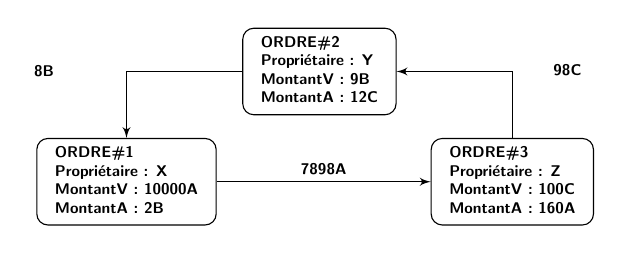
\begin{tikzpicture}[
    auto, 
    node distance=2cm,
    >=latex',
    font=\bfseries\footnotesize\sffamily,
    order/.style={
		scale=0.7,
		rectangle,
		rounded corners,
		draw=black, 
		text centered,
%		text width=5cm,
		minimum height=12mm,
		fill=white
	},
	label/.style={
		scale=0.7
	}
  ]
    % We start by placing the blocks

  \node [order] (order2) 
 {%
 \begin{tabular}{l}
  \textbf{ORDRE\#2}\\
  \textbf{Propriétaire : Y}\\
  \textbf{MontantV : 9B}\\
  \textbf{MontantA : 12C}
 \end{tabular}
 };
 
  \node [order, below of=order2, xshift=-3.5cm] (order1) 
 {%
 \begin{tabular}{l}
  \textbf{ORDRE\#1}\\
  \textbf{Propriétaire : X}\\
  \textbf{MontantV : 10000A}\\
  \textbf{MontantA : 2B}
 \end{tabular}
 };
 
 
  \node [order, below of=order2, xshift=3.5cm] (order3) 
 {%
 \begin{tabular}{l}
  \textbf{ORDRE\#3}\\
  \textbf{Propriétaire : Z}\\
  \textbf{MontantV : 100C}\\
  \textbf{MontantA : 160A}
 \end{tabular}
 };
 
 \draw [draw,->] (order1) -- node [label] {\textbf{7898A}} (order3);
 \draw [draw,->] (order2) -| node [label, xshift=-1.8cm] {\textbf{8B}} (order1);
 \draw [draw,->] (order3) |- node [label, xshift=1cm, yshift=0.24cm] {\textbf{98C}} (order2);

\end{tikzpicture}

\caption{Un anneau d'ordres de 3 ordres}
\label{fig:ring}
\end{figurehere}
\end{center}


La figure ci-dessus illustre un anneau de 3 ordres. Dans un anneau, le token à vendre (\verb|tokenV|) d'un ordre est le token à acheter (\verb|tokenA|) d'un autre ordre, et ce pour chaque ordre. Une boucle est créée, permettant à chaque token d'être échangé sans avoir besoin d'avoir un ordre opposé pour la paire désirée. Bien entendu, des ordres d'une seule paire peuvent toujours être exécutés, mais c'est en fin de compte un cas particulier d'un anneau d'ordres (anneau à deux ordres). 

\begin{definition}[order-ring] Soient $C_{0}$, $C_{1}$, $\cdots$, $C_{n-1}$  $n$ tokens distincts, soient $O_{0\rightarrow 1}$, $\cdots$, $O_{i\rightarrow i\oplus 1}$, $\cdots$, $O_{n-1 \rightarrow 0}$  $n$ ordres. Ces ordres peuvent former un anneau d'ordres pour un échange:
$$O_{0\rightarrow 1} \rightarrow \cdots \rightarrow O_{i\rightarrow i\oplus 1} \rightarrow \cdots \rightarrow O_{n-1\rightarrow 0} \text{, }$$
avec $n$ la longueur de l'anneau, et $i\oplus 1 \equiv i+1 \mod n$.
\end{definition}

Un anneau d'ordres est considéré valide lorsque toutes les transactions qui le composent peuvent être exécutées à un taux de change au moins aussi avantageux que celui demandé implicitement par l'utilisateur dans son MOUD. Pour vérifier la validité d'un anneau d'ordres, les smart contracts du protocole Loopring doivent recevoir l'anneau d'un mineur d'anneaux dont le produit des taux de changes originaux est supérieur ou égal à 1.

Supposons que Alice et Bob veulent échanger leurs tokens \verb|A| et \verb|B|. Alice a 15 tokens \verb|A| et aimerait en échange 4 tokens \verb|B|; Bob a 10 tokens \verb|B| et aimerait 30 tokens \verb|A| en échange.

Qui vend et qui achète ? Cela va seulement dépendre de l'actif sur lequel nous allons nous baser pour déterminer un prix. Si le token \verb|A| sert de référence, alors Alice achète B \verb|B| au prix de ${15 \over 4} = 3.75$\verb|A|, tandis que Bob vend 10 tokens \verb|B| au prix de  ${30 \over 10} = 3.00$\verb|A|. Inversement, si on prend le token \verb|B| pour référence, alors on peut dire qu'Alice vend \verb|A| au prix de ${4\over 15}=0.26666667$\verb|B| et Bob achète 10 tokens \verb|A| à ${10 \over 30}=0.33333334$\verb|B|. Ainsi, qui est l'acheteur ou le vendeur est purement arbitraire.

Dans la première situation, Alice est prête à payer un prix plus élevé ($3.75$\verb|A|) que celui auquel Bob vend ses tokens ($3.00$\verb|A|), alors que dans le second cas, Bob est prêt à payer un prix plus élevé ($0.33333334$\verb|B|) que celui auquel Alice vend les siens ($0.26666667$\verb|B|). Il est évident qu'un échange peut être conclu dès lors que l'acheteur est prêt à payer un prix au moins aussi élevé que celui du prix de vente du vendeur.

\begin{equation}
{{15\over 4} \over {30\over 10}} = {{10\over 30} \over {4\over 15}}={15 \over 4} \cdot {10 \over 30} = 1.25 > 1
\end{equation}

Par conséquent, pour un ensemble $n$ d'ordres à exécuter, entièrement ou partiellement, nous avons besoin de déterminer si le produit de chacun des taux de changes des ordres d'achat est supérieur à 1. Si tel est le cas, tous les ordres $n$ peuvent être partiellement ou totalement exécutés \cite{supersymmetry}.

Si on ajoute un troisième acteur, Charlie, dans le contexte suivant : Alice veut échanger $x_1$ tokens \verb|A| contre $y_1$ token \verb|B|, Bob $x_2$ tokens \verb|B| contre $y_2$ token \verb|C|, et Charlie $x_3$ tokens \verb|C| contre $y_3$ tokens \verb|A|. Les tokens requis sont présents, et l'échange est possible si :

\begin{equation}
{{x1 \cdot x_2 \cdot x_3 \over y_1 \cdot y_2 \cdot y_3} \geq 1}
\end{equation}


La rubrique \ref{anatomy} fournit davantage de détails sur les ordres Loopring.


\section{Participants à l'Ecosystème\label{sec:ecosystem}}
Ensemble, les participants à l'écosysteme fournissent toutes les fonctionnalités qu'un marché centralisé peut offrir. 

\begin{itemize}

\item \textbf{Portefeuilles} : Un service ou une interface de portefeuille qui donne aux utilisateurs l'accès à leurs tokens, et un moyen de passer des ordres sur le réseau Loopring. Les portefeuilles sont récompensés pour leur passage d'ordres grâce à un partage des commissions avec les mineurs d'anneaux (voir section \ref{sec:token}). En sachant que le futur de l'échange au lieu de manière sécurisé directement via les portefeuilles, connecter ces réserves de liquidité avec notre protocole est primordial.

\item \textbf{Blockchain de regroupement pour le partage de liquidité/maille de relais} : Une maille de relais pour les ordres et le partage de liquidités. Lorsque les nœuds exécutent le code des relais Loopring, ils ont la possibilité de rejoindre un réseau existant et de partager la liquidité sur une blockchain de regroupement. La blockchain de regroupement que nous sommes en train de construire permet un partage des ordres quasiment en temps réel (blocs de 1 à 2 secondes) dès la première implémentation, et ordre l'historique trop ancien pour permettre un téléchargement plus rapide par les nouveaux nœuds. A noter que les relais ne sont pas contraints de se joindre à ce regroupement; ils peuvent agir seuls et ne pas partager la liquidité avec les autres, ou, ils peuvent décider de créer et gérer leur propre réseau de partage de liquidité.

\item \textbf{Relais/Mineurs d'anneaux} : Les relais sont des nœuds qui reçoivent des ordres des portefeuilles ou de la maille de relais, et maintiennent des carnets d'ordres publics et l'historique des échanges, et facultativement, publient les ordres aux autres relais (via n'importe quel support off-chain) et/ou nœuds de la maille de relais. Miner des anneaux d'ordres est une fonctionnalité -- et non une nécessité -- pour les relais. C'est une tâche conséquente en terme de calculs, et est effectuée entièrement off-chain. Nous appelons les relais avec la fonctionnalité de minage d'anneaux activée les \enquote{Mineurs d'Anneaux}. Ils produisent les anneaux d'ordre en rapiéçant des ordres disparates. Les relais sont libres de choisir (1) comment ils souhaitent communiquer avec les autres, (2) comment ils construisent leurs carnets d'ordres, et (3) comment ils minent leurs anneaux (algorithmes de minage).

\item \textbf{Smart Contracts du Protocole Loopring (SCPL)} : Un ensemble de smart contracts public et gratuits qui vérifient les anneaux d'ordres reçus des mineurs d'anneaux, règlent et transfèrent sans tiers de confiance les tokens de la part des utilisateurs, récompensent les mineurs et les portefeuilles avec des commissions, et publient des évènements. Les explorateurs de relais et d'ordres écoutent ces évènement pour maintenir leur carnets d'ordres et l'historique des échanges à jour.

\item \textbf{Services de tokénisation d'actifs (STA)} : Une passerelle pour les actifs qui ne peuvent être échangés directement avec Loopring. Ce sont des services centralisés gérés par des entreprises ou des organisations de confiance. Les utilisateurs déposent des actifs (réels, fiat, ou des tokens d'autres blockchains) et en échange obtiennent des tokens qui peuvent être réclamés lors du dépôt. Loopring n'est pas un protocole d'échange cross-chain (jusqu'à ce qu'une telle solution existe), mais les STA permettent l'échange de tokens ERC20 \cite{ERC20} avec des actifs physique aussi bien qu'avec des tokens issus d'autres blockchains. 

\end{itemize}


\section{Processus d'échange\label{sec:process}}



\begin{enumerate} 


\item \textbf{Protocole d'autorisation}: Sur la figure \ref{fig:process}, l'utilisateur \verb|Y| qui veut échanger des tokens autorise le SCPL à traiter un \verb|montantV| du token \verb|B| que l'utilisateur veut vendre. Cela ne verrouille pas les tokens de l'utilisateur, qui reste libre de les transférer tant que l'ordre n'est pas exécuté.

\item \textbf{Création de l'ordre} : Le taux actuel et le carnet d'ordres pour le token \verb|B| contre le token \verb|C|, sont fournis par les relais ou d'autres agents connectés au réseau, tels que les explorateurs de carnets d'ordres. L'utilisateur \verb|Y| passe un ordre (ordre à cours limité) en spécifiant le \verb|montantV| et le  \verb|montantA|et autres paramètres via n'importe quelle interface de portefeuille intégrée. Un montant de LRx peut être adjointe à l'ordre comme commission pour les mineurs d'anneaux; plus les commissions en LRx sont élevés, plus la chance d'être traité tôt par les mineurs d'anneaux est élevée. Le hachage de l'ordre est signé avec la clé privée de \verb|Y|.

\item \textbf{Publication d'ordre} : Le portefeuille envoie l'ordre et sa signature à au moins un relais. Les relais mettent à jour leurs carnets d'ordres. Le protocole ne requiert pas que les carnets d'ordres soient construits d'une manière particulière, de type premier arrivé premier servi. A la place, les relais ont le pouvoir de prendre leurs propres décisions de design dans la construction de leurs carnets d'ordres.

\item \textbf{Partage de liquidité} : Les relais publient les ordres aux autres relais par n'importe quel moyen de communication. Encore une fois, une certaine flexibilité est offerte quant à la manière dont les nœuds interagissent. Pour permettre un certain niveau d'interconnectivité, une maille de nœuds de partage de liquidité utilisant une blockchain de regroupement est intégrée par défaut. Comme mentionné dans la section précédente, cette maille de relais est optimisée pour la vitesse et l'intégration.

\begin{center}
\begin{figurehere}
\centering
\tikzstyle{block} = [draw, fill=blue!20, rectangle, 
    minimum height=3em, minimum width=6em]
\tikzstyle{sum} = [draw, fill=blue!20, circle, node distance=1cm]
\tikzstyle{input} = [coordinate]
\tikzstyle{output} = [coordinate]
\tikzstyle{pinstyle} = [pin edge={to-,thin,black}]

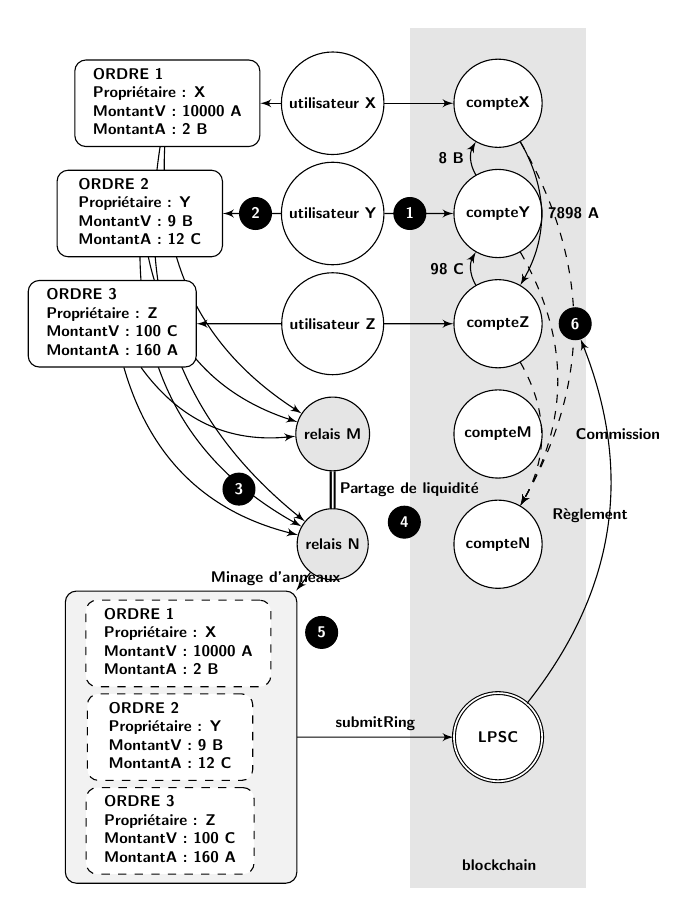
\begin{tikzpicture}[
    auto, 
    scale=0.7,
    node distance=2cm,
    >=latex',
    font=\bfseries\footnotesize\sffamily,
    order/.style={
		rectangle,
		scale=0.7,
		rounded corners,
		draw=black, 
		text centered,
%		text width=5cm,
		minimum height=12mm,
		minimum width=30mm,
		fill=white
	},
	role/.style={
		circle,
		scale=0.7,
		draw=black, 
		text centered,
%		text width=5cm,
		minimum height=12mm,
		minimum width=12mm,
		fill=white
	},
	steps/.style={
		circle,
		scale=0.7,
		draw=black, 
		text centered,
%		text width=5cm,
%		minimum height=12mm,
%		minimum width=12mm,
		fill=black,
		text=white
	},
	account/.style={
		circle,
		scale=0.7,
		draw=black, 
		text centered,
%		text width=5cm,
		minimum height=16mm,
		minimum width=16mm,
		fill=white
	},
	label/.style={
	  scale=0.7
    }
  ]

 
 \node [role] (user1)  {utilisateur X};
 \node [role, below of=user1] (user2)  {utilisateur Y};
 \node [role, below of=user2] (user3)  {utilisateur Z};
 \node [role, below of=user3, fill=gray!20] (relay1)  {relais M};
 \node [role, below of=relay1, fill=gray!20] (relay2)  {relais N};

 
 \node [order, left of=user1, xshift=-1cm] (order1) 
 {%
 \begin{tabular}{l}
  \textbf{ORDRE 1}\\
  \textbf{Propriétaire : X}\\
  \textbf{MontantV : 10000 A}\\
  \textbf{MontantA : 2 B}
 \end{tabular}
 };
 
 \draw [draw, ->]  (user1) -- (order1) [label]{};
 \draw [bend right,->] (order1) to node [auto, scale=0.7] {} (relay1);
 \draw [bend right,->] (order1) to node [auto, scale=0.7] {} (relay2);
% \draw [draw, ->]  (order1) |- (relay1) [label]{};
% \draw [draw, ->]  (order1) |- (relay2) [label]{};
 
 \node [order,left of=user2, xshift=-1.5cm] (order2) 
 {%
 \begin{tabular}{l}
  \textbf{ORDRE 2}\\
  \textbf{Propriétaire : Y}\\
  \textbf{MontantV : 9  B}\\
  \textbf{MontantA : 12 C}
 \end{tabular}
 };
 \draw [draw, ->]  (user2) -- (order2) [label]{};
 \draw [bend right,->] (order2) to node [auto, scale=0.7] {} (relay1);
 \draw [bend right,->] (order2) to node [auto, scale=0.7] {} (relay2);
% \draw [draw, ->]  (order2) |- (relay1) [label]{};
% \draw [draw, ->]  (order2) |- (relay2) [label]{};
% 
\node [order, left of=user3, xshift=-2cm] (order3) 
 {%
 \begin{tabular}{l}
  \textbf{ORDRE 3}\\
  \textbf{Propriétaire : Z}\\
  \textbf{MontantV : 100 C}\\
  \textbf{MontantA : 160 A}
 \end{tabular}
 };
 \draw [draw, ->]  (user3) -- (order3) [label]{};
 \draw [bend right,->] (order3) to node [auto, scale=0.7] {} (relay1);
 \draw [bend right,->] (order3) to node [auto, scale=0.7] {} (relay2);
% \draw [draw, ->]  (order3) |- (relay1) [label]{};
% \draw [draw, ->]  (order3) |- (relay2) [label]{};
 
% // The Ring
\node [order, 
yshift=-1.5cm,
xshift=-2.75cm,
below of=relay2,
fill=gray!10,
minimum width=4.2cm,
minimum height=5.3cm] (ring) {};


\node [order, dashed, below of=relay2,yshift=0.2cm,xshift=-2.8cm] (order11) 
 {%
 \begin{tabular}{l}
  \textbf{ORDRE 1}\\
  \textbf{Propriétaire : X}\\
  \textbf{MontantV : 10000 A}\\
  \textbf{MontantA : 2 B}
 \end{tabular}
 };
 \node [order, dashed,below of=order11,xshift=-0.15cm,yshift=0.3cm] (order21) 
 {%
 \begin{tabular}{l}
  \textbf{ORDRE 2}\\
  \textbf{Propriétaire : Y}\\
  \textbf{MontantV : 9  B}\\
  \textbf{MontantA : 12 C}
 \end{tabular}
 };
\node [order, dashed,below of=order21,xshift=0cm,yshift=0.3cm] (order31) 
 {%
 \begin{tabular}{l}
  \textbf{ORDRE 3}\\
  \textbf{Propriétaire : Z}\\
  \textbf{MontantV : 100 C}\\
  \textbf{MontantA : 160 A}
 \end{tabular}
 };
 
 % // The blockchain
\node [
rectangle,
fill=gray!20, 
right of=user1,
yshift=-4.5cm,
xshift=0.1cm,
scale=0.7,
minimum width=3.2cm,
minimum height=15.6cm] (blockchain) {\parbox[b][15cm]{1.3cm}{blockchain}};
% blockchain accounts
  \node [account, right of=user1, xshift=1cm] (account1)  {compteX};
  \node [account, right of=user2, xshift=1cm] (account2)  {compteY};
  \node [account, right of=user3, xshift=1cm] (account3)  {compteZ};
  \node [account, right of=relay1, xshift=1cm] (account4)  {compteM};
  \node [account, right of=relay2, xshift=1cm] (account5)  {compteN};
  \node [account, double, below of=account5, yshift=-1.5cm] (psc)  {LPSC};
  
 \draw [draw, ->]  (user1) -- (account1) [label]{};
 \draw [draw, ->]  (user2) -- (account2) [label]{};
 \draw [draw, ->]  (user3) -- (account3) [label]{};
% \draw [draw, ->]  (relay1) -- (account4) [label]{};
% \draw [draw, ->]  (relay2) -- (account5) [label]{};
 \draw [draw, double, thick]  (relay1) to node [auto, scale=0.7] {Partage de liquidité}  (relay2) [label]{};
% \draw [draw, ->]  (relay1) -- (ring) [label]{};
 \draw [draw, ->]  (relay2) to node [auto, scale=0.7, xshift=-1.8cm, yshift=0.3cm] {Minage d'anneaux}  (ring) [label]{};
 \draw [draw, ->]  (ring) to node [auto, scale=0.7] {submitRing} (psc) [label]{};
 
 \draw [bend left,->] (account1) to node [auto, scale=0.7] {\textbf{7898 A}} (account3);
 \draw [bend left,->] (account2) to node [auto, scale=0.7] {\textbf{8 B}} (account1);
 \draw [bend left,->] (account3) to node [auto, scale=0.7] {\textbf{98 C}} (account2);
 
 \draw [bend left,->, dashed] (account1) to node [auto, scale=0.7] {} (account5);
 \draw [bend left,->, dashed] (account2) to node [auto, scale=0.7] {} (account5);
 \draw [bend left,->, dashed] (account3) to node [auto, scale=0.7, xshift=.5cm] {\textbf{Commission}} (account5);
  
  
% \draw [draw,->] (order1) -- node [label] {\textbf{7898 A}} (order3);
% \draw [draw,->] (order2) -| node [label, xshift=-1.8cm] {\textbf{8 B}} (order1);
% \draw [draw,->] (order3) |- node [label, xshift=1cm, yshift=0.24cm] {\textbf{98 C}} (order2);

\node [steps, right of=user2, xshift=-0.6cm] () {1};
\node [steps, left of=user2, xshift=0.6cm] () {2};
\node [steps, left of=relay2, xshift=0.3cm, yshift=1cm] () {3};
\node [steps, left of=relay1, xshift=3.3cm, yshift=-1.6cm] () {4};
\node [steps, below of=relay2, xshift=-0.2cm, yshift=0.4cm] () {5};
\node [steps, right of=account3, xshift=-0.6cm] (step5) {6};

 \draw [bend right, ->]  (psc) to node [auto, scale=0.7, xshift=0.5cm] {Règlement} (step5) [label]{};
 
\end{tikzpicture}

\caption{Processus d'échange avec Loopring}
\label{fig:process}
\end{figurehere}
\end{center}



\item \textbf{Ring-Mining (Order Matching)} : Les mineurs d'anneaux tentent d'exécuter les ordres intégralement ou partiellement au cours actuel ou à un meilleurs cours en les appariant avec plusieurs ordres. Les mineurs d'anneaux sont la raisons principale pour laquelle le protocole est capable de fournir une liquidité élevée sur n'importe quelle paire. Si le cours exécuté est meilleurs que celui que l'utilisateur Y avait spécifié, la marge est partagée par tous les ordres de l'anneau. A titre de récompense, le mineur d'anneaux choisit entre obtenir une part de la marge (partage de marge avec une retour des LRx à l'utilisateur), ou garder la commission fixe en LRx.

\item \textbf{Vérification \& Règlement} : L'anneau d'ordres est reçu par le SCPL. Il effectue plusieurs vérifications sur les données fournies par le mineur d'anneaux et détermine si l'anneau d'ordres peut être réglé intégralement ou partiellement (selon le taux d'exécution des ordres dans l'anneau et les tokens dans les portefeuilles des utilisateurs). Si tous les critères sont remplis, le contrat effectue le transfert de chaque token aux utilisateurs et paie le mineur d'anneaux et les commissions du portefeuille à la fois. Si de solde de l'utilisateur \verb|Y| tel que déterminé par le LPSC n'est est pas suffisant, l'ordre sera considéré comme "réduit" : un ordre réduit sera automatiquement replacé à sa taille originale si les fonds suffisant sont déposés sur son adresse, contrairement à une annulation qui est une opération manuelle et qui n'est pas réversible.


\end{enumerate}





%
%\end{multicols}
%
%\begin{center}
%\begin{figurehere}
%\includegraphics[height=8cm]{images/en_protocol.png}
%\caption{Loopring Trading Process}
%\label{fig: Loopringrotocol}
%\end{figurehere}
%\end{center}
%
%\begin{multicols}{2}

\section{Flexibilité opérationnelle\label{sec:business_model}}
Il est important de souligner que les normes ouvertes de Loopring donnent aux participants une flexibilité importante dans leur manière d'opérer. Les différents acteurs sont libres d'implémenter de nouveaux modèles économiques et de créer de la valeur supplémentaire pour les utilisateurs, en engrangeant des commissions sous forme de LRx basées sur le volume d'échange ou d'autres métriques de leur choix. L'écosystème Loopring est modulaire et prévu pour supporter une multitude d'applications.


\subsection{Carnet d'ordres\label{sec:order_book}}
Les relais peuvent concevoir leur carnet d'ordres de n'importe quelle façon tant qu'ils affichent et apparient les ordres des utilisateurs. La première implémentation de notre propre carnet d'ordres suit le modèle OTC (over-the-counter, hors côte en français), dans lequel les ordres à cours limité sont ordonnés uniquement selon leur prix. En d'autres termes, la date et l'heure à laquelle l'ordre a été passé n'a pas d'importance. Cependant, un relai est libre de concevoir ses carnets d'ordres de manière à émuler le comportement typique d'un marché d'échange centralisé, où les ordres sont ordonnés par prix et pour un prix donné par ordre chronologique. Si un relais était tenté d'offrir ce type de carnet d'ordres, il pourrait l'intégrer dans un portefeuille et faire en sorte que les ordres émanant de ce portefeuille soient envoyé uniquement à ce relais, qui pourrait ensuite apparier les ordres basés sur leur date et heure. Toutes les configurations sont possibles.

Alors que d'autres protocoles de DEX nécessitent que les relais aient des ressources propres (un solde initial de tokens pour placer les ordres de l'acheteur), les relais de Loopring ont seulement besoin d'ordres correspondants pour exécuter un échange, et ce sans le moindre token initial.

\subsection{Partage de Liquidité\label{sec:liquidity_sharing}}
Les relais sont libres de décider comment se partager la liquidité entre eux. Notre blockchain de regroupement n'est que l'une des solutions possibles, et l'écosystème peut choisir ses propres moyens de communication. Hormis se joindre à une blockchain de regroupement, ils peuvent aussi construire et gérer la leur, créer des règles et des incitations monétaires comme bon leur semble. Les relais peuvent aussi fonctionner seuls, comme dans le cas de l'implémentation des portefeuilles de type ''time-sensitive''. Bien entendu, il existe des avantages certains à communiquer avec d'autres relais dans le but d'obtenir des effets de réseaux. Cependant, des modèles économiques différents pourraient mériter un design de partage de liquidité qui leur est propre et un partage de commissions de nombreuses façons.

\section{Spécifications du Protocole\label{sec:protocol}}

\subsection{Anatomie d'un ordre\label{anatomy}}
Un ordre est un ensemble de données décrivant les intentions d'échange d'un utilisateur. Un ordre Loopring est donné selon le Modèle d'Ordre Unidirectionnel, ou MOUD, sous la forme suivante :

\begin{verbatim}
  message Order {
    address protocol;
    address owner;
    address tokenS;  
    address tokenB;
    uint256 amountS;
    uint256 amountB;
    unit256 lrcFee
    unit256 validSince; // Secondes depuis l'epoch
    unit256 validUntil; // Secondes depuis l'epoch
    uint8   marginSplitPercentage;  // [1-100]
    bool    buyNoMoreThanAmountB;
    uint256 walletId;
    // Adresse pour le Dual-Authoring 
    address authAddr;
   	// v, r, s font partie de la signature
    uint8   v;       
    bytes32 r;
    bytes32 s;
    // Clé privée du Dual-Authoring ,
    // pas utilisée pour signer le hash de l'ordre,
    // donc elle n'est PAS signée.
    string  authKey;          
  }
\end{verbatim}


Pour s'assurer de l'origine d'un ordre, ce dernier est signé avec le hash de ses paramètres, en excluant \verb|authAddr|, et avec la clé privée de l'utilisateur. Le paramètre \verb|authAddr| est utilisé pour signer des anneaux d'ordres dont cet ordre fait partie, ce qui empêche les tentatives de front-running. Veuillez vous référer à la section \ref{sec:dual_authoring} pour plus de détails. La signature est représentée avec les champs \verb|v|, \verb|r|, et \verb|s|, et est envoyée sur le réseau aux côtés des paramètres de l'ordre. Cela garantit l'immuabilité de l'ordre tout au long de son existence. Bien que l'ordre ne change jamais, le protocole peut toujours déterminer son état actuel d'après le solde de son adresse ainsi que d'autres variables.


Le MOUD n'inclut pas de prix (qui est par nature un nombre à virgule flottante), mais utilise plutôt le terme \verb|taux| ou $r$, égal à \verb|MontantV|/\verb|MontantA|. Le taux n'est pas un nombre à virgule flottante, mais une formule qui sera seulement évaluée à la demande avec d'autres entiers non-signés pour pouvoir garder tous les résultats intermédiaires sous la forme d'entiers non-signés et améliorer ainsi la précision des calculs. 

\subsubsection{Montants d'achat}

Lorsqu'un mineur d'anneaux arrive à compléter un anneau d'ordres, il est possible qu'un meilleur taux soit exécutable, permettant ainsi aux utilisateur de recevoir plus de \verb|TokenB| que le \verb|montantA| qu'ils avaient demandé. Cependant, si \verb|buyNoMoreThanAmountB| (''pas plus que tant de tokens B'' en français) est défini à \verb|True|, le protocole s'assure que les utilisateurs ne reçoivent pas plus que  \verb|montantA| de \verb|tokenB|. Ainsi, le paramètre \verb|buyNoMoreThantokenB| du MOUD détermine lorsqu'un ordre est considéré comme entièrement exécuté. Le paramètre \verb|buyNoMoreThantokenB| applique un plafond soit sur \verb|montantV| soit sur \verb|montantA|, et permet aux utilisateurs plus de finesse dans l'expression de leurs intentions d'échange que les ordres traditionnels de type achat/vente.

Par exemple : avec \verb|montantV| = 10 et \verb|montantA| = 2, le taux est $r$ = 10/2 = 5. Par conséquent, l'utilisateur est prêt à vendre 5 \verb|TokenV| par \verb|TokenA|. Le mineur d'anneaux trouve un anneau avec un taux de 4, permettant à l'utilisateur de recevoir 2.5 \verb|tokenA| au lieu de 2. Mais si l'utilisateur souhaite seulement 2 \verb|tokenA| et définit \verb|buyNoMoreThanAmountA| à \verb|True|, le LPSC effectue une transaction à un taux de 4 \verb|tokenV| pour chaque \verb|tokenA| pour un total de 8 \verb|tokenV|, économisant effectivement 2 \verb|tokenV|. Notons au passage que ce modèle ne prend pas en compte les commissions (voir section \ref{sec:fee_model}).

En effet, si on utilise:


\begin{verbatim}
	      Order(montantV,tokenV,
	            montantA,tokenA,
	            buyNoMoreThantokenA)
\end{verbatim}

pour exprimer un ordre sous une forme simplifiée. Avec une paire ETH/USD sur un marché centralisé, le modèle achat/vente traditionnel peut exprimer les premièr et troisième ordres ci-dessous mais pas les deux autres : 

\begin{enumerate}
	\item Vendre 10 ETH à 300 USD/ETH. Cet ordre peut être exprimé comme: \verb|Order(10, ETH, 3000, USD, Faux)|.
	\item Vendre ETH à 300 USD/ETH to get 3000 USD. Cet ordre peut être exprimé de la manière suivante: \verb|Order(10, ETH, 3000, USD, Vrai)|.
	\item Acheter 10 ETH à 300 USD/ETH, cet ordre peut être exprimé de la manière suivante : \verb|Order(3000, USD, 10, ETH, Vrai)|.
	\item Dépenser 3000 USD pour acheter d'autant d'ETH que possible à 300 USD/ETH, cet ordre peut être exprimé de la manière suivante: \verb|Order(3000, USD, 10, ETH, Faux)|.
\end{enumerate}



\subsection{Vérification d'un anneau\label{sec:ring_verification}}

Les smart contracts de Loopring n'effectuent pas les calculs de taux ou de montants, mais doivent recevoir et vérifier les valeurs que les mineurs d'anneaux. Ces calculs sont faits par les mineurs d'anneaux pour deux raisons majeures : (1) le langage de programmation utilisé pour l'écriture des smart contracts, comme solidity\cite{dannen2017introducing} sur Ethereum, ne supporte pas les calculs à virgule flottante, particulièrement pour $pow(x, 1/n)$ (calcul de la racine n-ième d'un nombre à virgule flottante), et (2) il est souhaitable que le calcul soit effectué off-chain pour alléger  le coût et l'effort sur la blockchain.


\subsubsection{Validation de sous-anneaux\label{sec:sub_ring_check}}
Cette étape empêche les arbitrageurs de réaliser une marge injustement sur un anneau d'ordres en implémentant de nouveaux ordres en son sein. L'idée est que dès qu'un ordre valide est trouvé par un mineur d'anneaux, il pourrait être tentant d'ajouter de nouveaux ordres à l'anneau pour absorber toute marge des utilisateurs (rabais sur leur taux). Comme illustré sur la figure \ref{fig:subring} ci-dessus, un calcul précis de $x1$, $y1$, $x2$ and $y2$ rendra le produit du taux de tous les ordres exactement égal à 1 ce qui empêche tout rabais sur le taux de change. 

\begin{center}
\begin{figurehere}
\centering
\tikzstyle{block} = [draw, fill=blue!20, rectangle, 
    minimum height=3em, minimum width=6em]
\tikzstyle{sum} = [draw, fill=blue!20, circle, node distance=1cm]
\tikzstyle{input} = [coordinate]
\tikzstyle{output} = [coordinate]
\tikzstyle{pinstyle} = [pin edge={to-,thin,black}]

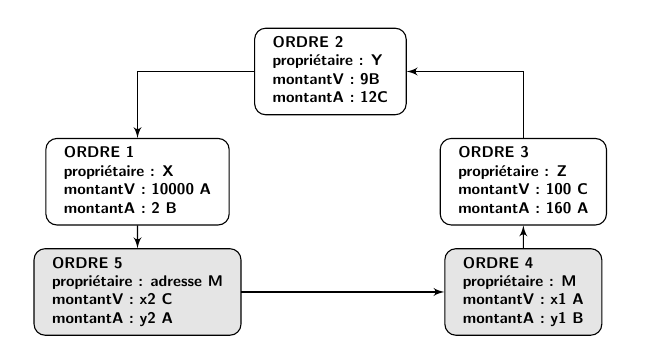
\begin{tikzpicture}[
    auto, 
    node distance=2cm,
    >=latex',
    font=\bfseries\footnotesize\sffamily,
    order/.style={
		scale=0.7,
		rectangle,
		rounded corners,
		draw=black, 
		text centered,
%		text width=5cm,
		minimum height=12mm,
		fill=white
	},
	label/.style={
		scale=0.7
	}
  ]
    % We start by placing the blocks

  \node [order] (order2) 
 {%
 \begin{tabular}{l}
  \textbf{ORDRE 2}\\
  \textbf{propriétaire : Y}\\
  \textbf{montantV : 9B}\\
  \textbf{montantA : 12C}
 \end{tabular}
 };
 
  \node [order, below of=order2, xshift=-3.5cm] (order1) 
 {%
 \begin{tabular}{l}
  \textbf{ORDRE 1}\\
  \textbf{propriétaire : X}\\
  \textbf{montantV : 10000 A}\\
  \textbf{montantA : 2 B}
 \end{tabular}
 };
 
 
  \node [order, below of=order2, xshift=3.5cm] (order3) 
 {%
 \begin{tabular}{l}
  \textbf{ORDRE 3}\\
  \textbf{propriétaire : Z}\\
  \textbf{montantV : 100 C}\\
  \textbf{montantA : 160 A}
 \end{tabular}
 };
 
   \node [order, below of=order3, fill=gray!20] (order4) 
 {%
 \begin{tabular}{l}
  \textbf{ORDRE 4}\\
  \textbf{propriétaire : M}\\
  \textbf{montantV : x1 A}\\
  \textbf{montantA : y1 B}
 \end{tabular}
 };
 
 
  \node [order, below of=order1, fill=gray!20] (order5) 
 {%
 \begin{tabular}{l}
  \textbf{ORDRE 5}\\
  \textbf{propriétaire : adresse M}\\
  \textbf{montantV : x2 C}\\
  \textbf{montantA : y2 A}
 \end{tabular}
 };
 
 \draw [draw,->] (order1) -- node [label, xshift=-2cm] {} (order5);
 \draw [draw,->] (order2) -| node [label, xshift=-1.6cm] {} (order1);
 \draw [draw,->] (order3) |- node [label, xshift=1cm] {} (order2);
 \draw [draw,->] (order4) -- node [label, xshift=1.8cm] {} (order3);
 \draw [draw,->] (order5) -- node [label, yshift=0.2cm] {} (order4);
  
\end{tikzpicture}

\caption{Un anneau avec un sous-anneau}
\label{fig:subring}
\end{figurehere}
\end{center}

Ce mouvement n'implique aucun risque et n'apporte aucune valeur au réseau, et est considéré comme un comportement injuste par le mineur d'anneaux. Pour empêcher ceci, Loopring nécessite qu'un anneau valide ne peut contenir aucun sous-anneau. Pour ce faire, le LPSC s'assure qu'un token ne peut être plus d'une fois un token à vendre ou à acheter. Dans le diagramme ci-dessus, on voit que le token \verb|A| est vendu et acheté deux fois, ce qui devrait être rejeté.


\subsubsection{Vérification du taux d'exécution\label{sec:fill_rate_check}}

Le calcul des taux de change au sein de l'anneau d'ordres est effectué par les mineurs d'anneaux pour les raisons citées plus haut. C'est au LPSC de s'assurer qu'ils sont corrects. D'abord, il vérifie que le taux auquel le mineur d'anneaux peut exécuter chaque ordre est inférieur ou égal au taux initialement demandé par l'utilisateur. Cela apporte à l'utilisateur la garantie d'obtenir un taux au moins aussi bon que celui demandé. Dès que les taux de change sont confirmés, dans le cas où un taux meilleur que celui demandé est possible (il en résulte un rabais sur le taux demandé), le LPSC s'assure que tous les ordres composant l'anneau partagent le même taux réduit. Par exemple, si le rabais est de $\gamma$, alors le prix pour chaque ordre est de :

$r_{0\rightarrow 1} \cdot (1-\gamma)$, $r_{1\rightarrow 2} \cdot (1-\gamma)$, $r_{2 \rightarrow 0} \cdot (1-\gamma)$, et satisfait à l'équation suivante : 
\begin{equation}
r_{0\rightarrow 1} \cdot (1-\gamma)\cdot r_{1\rightarrow 2} \cdot (1-\gamma) \cdot r_{2 \rightarrow 0} \cdot (1-\gamma) = 1
\end{equation}
ainsi : 
\begin{equation}
\gamma = 1- \frac{1}{\sqrt[3]{r_{0\rightarrow 1} \cdot r_{1\rightarrow 2} \cdot r_{2\rightarrow 0}}}\text{.}
\end{equation}
Pour une transaction comprenant $n$ ordres, le \texttt{rabais} est égale à : 
\begin{equation}
\gamma = 1- \frac{1}{\sqrt[n]{\prod_{i=0}^{n-1} r^i}} \text{,}
\end{equation}

où $r^i$ est le taux d'éxécution du $i$-ième ordre. Bien sûr, les ordres ne peuvent être exécutés que lorsque $\gamma \ge 0$; et que le taux d'échange réel du $i$-ième ordre ($O^i$) soit $\hat{r^i} = r^i \cdot (1-\gamma)$, $\hat{r^i}\le r^i$.

Retournons à notre exemple précédent dans lequel Alice a 15 tokens \verb|A| and veut 4 tokens \verb|B| en échange, Bob a 10 tokens \verb|B| et veut 30 tokens \verb|A| en échange. Si le token \verb|A| sert de référence, alors Alice achète le token \verb|B| au taux $\frac{15}{4}$ = 3.75\verb|A|, tandis que Bob vend le token \verb|B| pour $\frac{30}{10}$ = 3.00\verb|A|. Pour calculer le taux de rabais : $\frac{150}{120}$ = 1.25 donc $\frac{1}{1.25}$ = 0.8 = $(1 - \gamma)^2$. Ainsi, le taux qui rend l''échange équitable pour les deux parties est $\sqrt{0.8}$ $\cdot$ 3.75 $\approx$ 3.3541 tokens \verb|A| par token \verb|B|.

Bob donne 4 tokens \verb|B| et reçoit 13.4164 tokens \verb|A|, soit davantage que les 12 auxquels il s'attendait. Alice reçoit 4 tokens \verb|B| comme convenu, mais ne donne que 13.4164 tokens \verb|A| en échange, moins que les 15 qu'elle était prête à payer pour ces 4 tokens.
A noter qu'une partie de cette marge servira à payer les commissions pour récompenser les mineurs et les portefeuilles. (voir section \ref{sec:fee_model}).

\subsubsection{Taux de d'exécution et annulation}

Un utilisateur peut annuler partiellement ou entièrement un ordre en envoyant une transaction particulière contenant tous les détails concernant l'ordre et les montants à annuler au LPSC. Ce dernier prend la transaction en compte, stocke le montant à annuler et émet un évènement de type \verb|OrderCancelled| (''ordre annulé'') au réseau. Le LPSC garde un historique des montants exécutés et annulés en stockant leur valeur avec pour identifiant le hash de l'ordre. Cette information est accessible publiquement et les évènements \verb|OrderCancelled| / \verb|OrderFilled| ('''ordre exécuté'') sont émis en cas de changement. Le suivi de ces valeurs est crucial pour le LPSC lors de l'étape du règlement des anneaux d'ordres.

Le LPSC permet aussi d'annuler tous les ordres de toutes les paires d'échanges en émettant un évènement \verb|OrdersCancelled| (''ordres annulés''), ou d'annuler tous les ordres pour une adresse donnée avec l'évènement \verb|AllOrdersCancelled| (''tous ordres annulés'').

\subsubsection{Mise à l'échelle des ordres \label{sec:order_scaling}}
Les ordres sont mis à l'échelle d'après l'historique des montants exécutés et annulés, et d'après le solde actuel des comptes expéditeurs. Le processus trouve les ordres avec le montant à exécuter le plus faible d'après les informations mentionnées précédemment, et les utilise comme référence pour mettre à l'échelle toutes les transactions de l'anneau d'ordres. 

Trouver l'ordre de plus faible valeur permet de savoir le volume à exécuter pour chaque ordre. Par exemple, si le $i$-ième ordre a la valeur la plus faible, alors le nombre de tokens vendus dans chaque ordre $\hat{s}$ et le nombre de tokens échangés $\hat{b}$ dans chaque ordre peut être calculé de la manière suivante :

\[
\begin{split}
&\hat{s}^{i}=\overline{s}_i\text{, } \hat{b}^{i}=\hat{s}^{i}/ \hat{r}^i\text{, }\text{;}\\
&\hat{s}^{i\oplus 1}=\hat{b}^i\text{, } \hat{b}^{i\oplus 1}=\hat{s}^{i\oplus 1}/ \hat{r}^{i\oplus 1}\text{;}\\
&\hat{s}^{i\oplus 2}=\hat{b}^{i\oplus 1}\text{, } \hat{b}^{i\oplus 2}=\hat{s}^{i\oplus 2}/ \hat{r}^{i\oplus 2}\text{;}\\
& ...
%\text{.}
\end{split}
\]
avec $\overline{s}_i$ représentant le solde une fois que les ordres ont été partiellement exécutés. 

Lors de l'implémentation, on peut sans aucun souci supposer que n'importe quel ordre dans l'anneau d'ordres a la valeur la plus faible, et ensuite itérer sur l'anneau d'ordres deux fois au plus pour calculer chaque volume d'exécution.

Exemple : Si le plus petit montant à être exécuté par rapport à l'ordre original est de 5\%, toutes les transactions de l'anneau d'ordres seront réduites à 5\%. Une fois les transactions exécutées, l'ordre qui était considéré comme ayant le plus faible montant restant à exécuter devrait être complètement exécuté.

\subsection{Règlement d'un anneau\label{sec:settlement}}

Si un anneau d'ordres remplit toutes les conditions requises, l'anneau d'ordres peut être fermé, et les transactions effectuées. Cela signifie que $n$ ordres forment un anneau d'ordres fermé, tel qu'illustré sur la figure 4:

\begin{center}
\begin{figurehere}
\centering
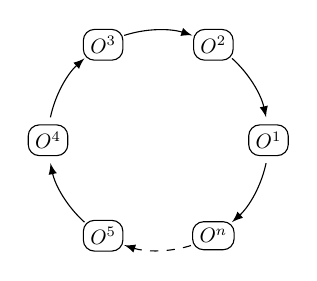
\begin{tikzpicture}[
circle/.style={
		scale=0.75,
		rounded corners,
		draw=black, 
		text centered,
		}
]

\def \n {6}
\def \m {4}
\def \radius {1.4cm}
\def \margin {12} % margin in angles, depends on the radius

\foreach \s in {1,...,\m}
{
  \node[draw, circle] at ({360/\n * (\s - 1)}:\radius) {$O^\s$};
  \draw[<-, >=latex] ({360/\n * (\s - 1)+\margin}:\radius) 
    arc ({360/\n * (\s - 1)+\margin}:{360/\n * (\s)-\margin}:\radius);
}

\node[draw, circle] at ({360/\n * 4}:\radius) {$O^5$};
  \draw[<-, dashed, >=latex] ({360/\n * 4+\margin}:\radius) 
    arc ({360/\n * 4+\margin}:{360/\n * (5)-\margin}:\radius);
    
\node[draw, circle] at ({360/\n * 5}:\radius) {$O^n$};
  \draw[<-, >=latex] ({360/\n * 5+\margin}:\radius) 
    arc ({360/\n * 5+\margin}:{360/\n * (6)-\margin}:\radius);


\end{tikzpicture}
\caption{Règlement d'un anneau}
\label{fig:settlement}
\end{figurehere}
\end{center}

Pour exécuter une transaction, le LPSC utilise le smart contract \verb|TokenTransferDelegate| ("délégation du transfert de tokens" en français). L'inclusion d'un tel système de délégation simplifie le protocole puisque tous les ordres ont seulement besoin d'autoriser le délégué au lieu des différentes versions potentielles du protocole.

Pour chaque ordre de l'anneau, un règlement de \verb|tokenV| est versé à l'ordre suivant ou précédant selon le type d'implémentation. Ensuite, la commission du mineur d'anneaux est versée selon le modèle de rémunération choisi par le mineur d'anneaux. Enfin, une fois toutes transactions effectuées, un évènement de type \verb|RingMined| ("AnneauMiné" en français) est émis.

\subsubsection{Evènements émis\label{sec:events}}

Le protocole émet des évènements qui permettent aux relais, aux explorateurs de carnets d'ordres, et aux autres acteurs de recevoir des mises à jour des carnets d'ordres de la manière la plus efficace possible. Les évènements émis sont les suivants :

\begin{itemize}
	\item \textbf{OrderCancelled} : Un ordre a été annulé.
	\item \textbf{OrdersCancelled} : Tous les ordres d'une paire d'une adresse sont annulés.
	\item \textbf{AllOrdersCancelled} : Tous les ordres de toutes les paires d'une adresse ont été annulés
	\item \textbf{RingMined} : Un anneau d'ordres a été exécuté. Cet évènement contient toutes les données relatives au transfert de chaque anneau intérieur. 
\end{itemize}


\section{Les Tokens LRx \label{sec:token}}
LRx est la notation générique de nos tokens. LRC est le token Loopring sur Ethereum, LRQ sur Qtum, et LRN sur NEO, etc. D'autres types de tokens LRx seront ajoutés à l'avenir lorsque Loopring sera déployé sur d'autres blockchains publiques.

\subsection{Modèle de commissions\label{sec:fee_model}} 
Lorsqu'un utilisateur passe un ordre, il précise une commission en LRx à payer au mineur d'anneaux, ainsi qu'un pourcentage de la marge effectuée sur l'ordre (\verb|marginSplitPercentage|) à laquelle le mineur d'anneaux peut prétendre. C'est ce qu'on appelle le partage de marge. La décision de choisir le type de commission (commission fixe ou marge partagée) appartient au mineur d'anneaux.

Le partage de marge peut être illustré de la manière suivante :

\begin{center}
\begin{figurehere}
\centering
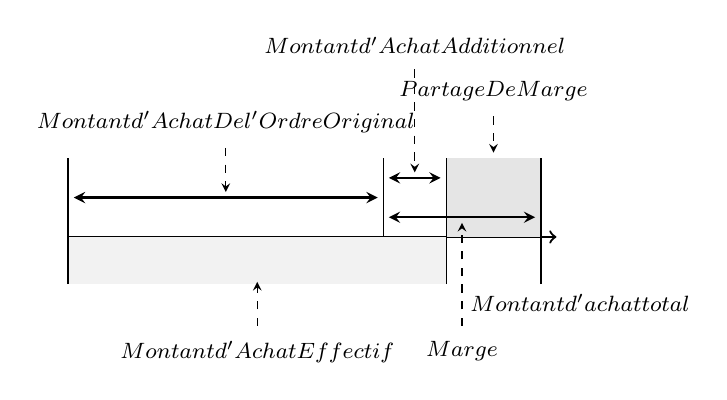
\begin{tikzpicture}[
scale=1,
font=\bfseries\footnotesize\sffamily,
classical/.style={thick,<->,shorten >=2pt,shorten <=2pt,>=stealth},
oneway/.style={->,dashed,shorten >=2pt,shorten <=2pt,>=stealth}
]
    % Draw axes
    \draw [->,thick] (0,1) node (yaxis) [above] {$$}
        |- (6.2,0) node (xaxis) [right] {$$};
        
    \draw
  	(4,0) coordinate (A)
  	(4,1) coordinate (A2)
  	(4.8,-0.6) coordinate (B)
  	(4.8,1) coordinate (B2)
  	(6,-0.6) coordinate (C)
  	(6,1) coordinate (C2);
  	
  	\fill [draw=none, fill=gray!20] 
    (4.8, 0) rectangle (6, 1);
    
  	\fill [draw=none, fill=gray!10] 
    (0, -0.6) rectangle (4.8, 0);

	\draw[thick] (0, -0.6) -- (0, 0.6) node[below]{$$};
  	\draw[thick, thin] (A) -- (A2) node[below]{$$};
  	\draw[thick, thin] (B) -- (B2) node[below]{$$};
  	\draw[thick] (C) node[below, xshift=0.5cm]{$Montant d'achat total$} -- (C2) ;
  	
  	\draw[classical] (0, 0.5) -> (4, 0.5) node[below]{$$};
  	\draw[classical] (4, 0.75) -> (4.8, 0.75) node[below]{$$};
%  	\draw[classical] (4.8, 0.5) -> (6, 0.5) node[below]{$$};
  	\draw[classical] (4, 0.25) -> (6, 0.25) node[below]{$$};

  	
  	\draw[oneway] (2, 1.2) node[above]{$Montantd'AchatDel'OrdreOriginal$} -- (2, 0.5);
  	\draw[oneway] (4.4, 2.2) node[above]{$Montantd'AchatAdditionnel$} -- (4.4, 0.75);
  	\draw[oneway] (5.4, 1.6) node[above]{$PartageDeMarge$} -- (5.4, 1);
  	\draw[oneway] (5, -1.2) node[below]{$Marge$} -- (5, 0.25);
  	\draw[oneway] (2.4, -1.2) node[below]{$Montantd'AchatEffectif$} -- (2.4, -0.5);



\end{tikzpicture}
\caption{Une marge partagée de 60\%}
\label{fig:marginsplit}
\end{figurehere}
\end{center}

Si la marge d'un anneaux d'ordres est trop faible, un mineur d'anneaux choisira la commission fixe en LRx. Si au contraire, la marge est conséquente au point que la marge partagée vaille plus que la commission fixe, alors le mineur d'anneaux choisira la marge partagée. Il existe une clause supplémentaire cependant : lorsque le mineur d'anneaux choisit la marge partagée, il doit payer une commission à l'utilisateur (le créateur de l'ordre), qui est égale au montant en LRx que l'utilisateur aurait dû payer au mineur d'anneaux comme commission. Cela porte le seuil à partir duquel le mineur d'anneaux choisira le partage de marge, au double de la commission fixe de l'ordre, ce qui tend à rendre plus fréquent le choix d'une commission fixe en LRx. Cela permet au mineur d'anneaux de lisser son revenu sur des anneaux d'ordres à faible marge, au détriment d'une marge partagée sur les anneaux d'ordres à marge élevée. Notre modèle se base sur notre prévision qu'avec la croissance du marché, les anneaux d'ordres à marge élevée seront de plus en plus rares, ce qui incitera des commissions fixes en LRx. 


Nous nous retrouvons avec le graphe suivant :

\begin{center}
\begin{figurehere}
\centering
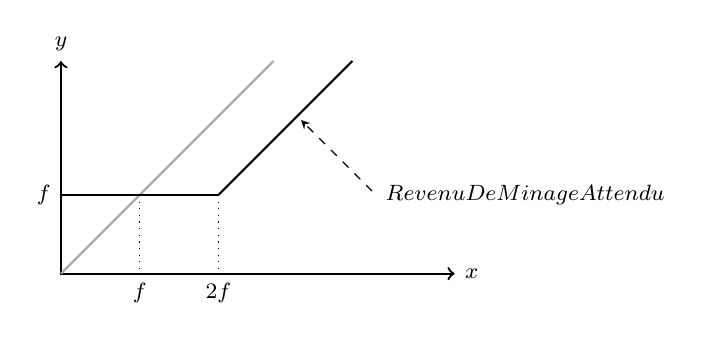
\begin{tikzpicture}[
font=\bfseries\footnotesize\sffamily,
oneway/.style={->,dashed,shorten >=2pt,shorten <=2pt,>=stealth},
scale=1]
    % Draw axes
    \draw [<->,thick] (0,2.7) node (yaxis) [above] {$y$}
        |- (5,0) node (xaxis) [right] {$x$};
        
    \draw
  	(1,1) coordinate (A)
  	(2,1) coordinate (B);
  	
  	
  	\draw[thick] (B) -- (3.7,2.7);
  	\draw[dotted] (B) -- (2,0) node[below] {$2f$};
  	\draw[dotted] (A) -- (1,0) node[below] {$f$};
  	\draw[thick,color=gray!70] (0,0) -- (2.7,2.7);
  	\draw[thick] (0,1) node[left] {$f$}--(B) node[     ]{$$};
 	\draw[oneway] (4,1) node[right]{$Revenu De Minage Attendu$} -- (3, 2);


\end{tikzpicture}
\caption{Le modèle Loopring's Fee Model}
\label{fig:feemodel}
\end{figurehere}
\end{center}


où $f$ est la commission fixe en LRx, $x$ est la marge partagée, $y$ est le revenu du minage. $y=max(f, x-f)$ comme indiqué par la ligne pleine; si la commission fixe pour l'ordre est de $0$, l'équation devient $y=max(0, x - 0)$ ce qui est peut être simplifié en $y=x$ tel qu'indiqué par la ligne grise.


On peut en déduire les points suivants :
\begin{enumerate}
	\item Si la marge partagée est de 0, les mineurs d'anneaux choisiront la commission fixe et sont toujours récompensés.
	\item Si la commission fixe est de 0, la ligne grise indique un revenu selon un modèle linéaire.
	\item Dès lors que la marge partagée est supérieure à deux fois la commission fixe, le mineur d'anneaux choisit la marge partagée, et paie un montant en LRx à l'utilisateur.
\end{enumerate}

Il faut garder à l'esprit que si la commission fixe est supérieure à zéro, quelle que soit l'option choisie par le mineur, il y aura toujours un transfert de LRx entre le mineur d'anneaux et l'émetteur de l'ordre. En effet, soit le mineur reçoit une commission en LRx, soit il paye la commission en retour à l'émetteur pour prendre la marge partagée.

Les mineurs d'anneaux partageront un certain pourcentage des commissions avec les portefeuilles. Lorsqu'un utilisateur place un ordre via un portefeuille et que cet ordre est exécuté, le portefeuille est récompensé par une portion des commissions ou du partage de marge. Bien que ce soit modulaire, et que des modèles économique et implémentations variés sont possibles, nous recommandons qu'un portefeuille reçoive environ 20 à 25\% des commmissions de l'ordre. Les portefeuilles sont une cible importante du protocole Loopring parce qu'ils sont nécessaires pour les utilisateurs, mais n'ont habituellement pas ou peu de sources de revenus.

\subsection{Gouvernance décentralisée}
Le protocole Loopring est un protocole social dans le sens où il dépend de la coopération des membres pour fonctionner efficacement dans un but commun. Ce n'est pas sans rappeler les autres protocoles cryptos en général, et en pratique, son utilité repose sur les mêmes mécanismes de coopération \cite{vitalikgovernance}, de stratégie dite "Grim Trigger equilibrium", et de rationalité limitée. A cette fin, les tokens LRx ne servent pas seulement au paiement des commissions liées aux échanges, mais aussi pour récompenser l'ensemble des participants au réseau. Un tel alignement est nécessaire à l'adoption de n'importe quel protocole, mais l'est d'autant plus pour les protocoles d'échange, étant donné que le succès est principalement lié à l'amélioration de la liquidité dans une écosystème décentralisé robuste.

Les tokens LRx seront aussi utilisés pour permettre des mises à jour du protocole via une gouvernance décentralisée. Les mises à jour des smart contracts seront gouvernées par les détenteurs de tokens LRx pour assurer la continuité et la sécurité du réseau, et aussi éviter les baisses de liquidité causées par les problèmes d'incompatibilité. Etant donné que les smart contracts ne peuvent être modifiés après leur déploiement, il existe un risque que les dApps ou les utilisateurs continuent d'interagir avec des versions obsolètes, s'excluant ainsi de l'utilisation des smart contracts à jour. La capacité d'être mis à jour est cruciale dans le succès du protocole car il n'a d'autre choix que de s'adapter aux demandes du marchés et aux blockchains sous-jacentes. La gouvernance décentralisée par les détenteurs de LRx permettra de mettre à jour les smart contracts sans interrompre l'utilisation des dApps ou des utilisateurs ni dépendre excessivement de l'abstraction de smart contracts. Au départ, cela se déroulera grâce à une simple signature multiple des smart contracts pour à terme évoluer vers un mécanisme de gouvernance de type DAO.

\section{Protection contre les fraudes et attaques}

\subsection{Protection contre le front-running\label{sec:dual_authoring}}

Dans le contexte des échanges décentralisés, le front-running correspond à la tentative pour quelqu'un de copier la solution d'un anneau d'un autre noeud, et de miner le bloc correspondant avant la transaction originale qui se trouve encore dans le pool de transactions en attente (mempool). Cela peut se réaliser en offrant une commission plus élevée (prix du gaz). Le principal procédé de front-running avec Loopring (et de n'importe quel protocole d'appariement d'ordres) est le vol d'ordre : lorsqu'un front-runner vole un ordre ou plus d'un anneau d'ordres en attente de validation de transaction ; et plus spécifique à Loopring, lorsqu'un front-runner vole l'anneau d'ordres entier d'une transaction en attente. 

Lorsqu'une transaction de type "submitRing" ("soumission d'anneau" en français) n'est pas encore confirmée et toujours dans le pool de transactions en attente, n'importe qui peut facilement détecter une telle transaction et remplacer le champ "\verb|minerAddress|" ("adresse du mineur" en français) avec leur propre adresse, la \verb|filcherAddress| (adresse du voleur en français), il est alors possible que le voleur puisse resigner l'ensemble avec l'adresse \verb|filcherAddress| pour remplacer la signature de l'anneau d'ordres original. Le voleur peut définir un prix du gaz plus élevé, et soumettre une nouvelle transaction en espérant que les mineurs l'incluent dans le premier bloc suivant au lieu de la transaction submitRing originale.

Les précédentes solutions pour à ce problème comportaient des inconvénients importants : nécessiter plus de transactions et ainsi coûter plus de gaz aux mineurs d'anneaux, et prendre au moins le double de blocs pour régler un anneau d'ordres. Notre nouvelle solution, le "Dual Authoring" \cite{dualauthor} ("double paternité" en français), implique un mécanisme à double niveau d'autorisation pour les ordres : un pour le règlement, un pour le minage d'anneaux. 

Processus de "Dual Authoring" :

\begin{enumerate}

	\item Pour chaque ordre, le code du portefeuille va générer un couple clé publique/clé privée aléatoire, et placer cette clé dans le JSON de l'ordre. Une alternative peut consister à prendre une adresse dérivée de la clé publique au lieu de la clé publique elle-même afin de réduire le nombre d'octets requis. Nous utilisons le champ \verb|authAddr| (adresse d'autorisation en français) pour stocker cette adresse, et \verb|authKey| pour stocker la clé privée correspondant à \verb|authAddr|).

	\item Le traitement du hash de l'ordre avec tous ses champs a lieu, à part \verb|r|, \verb|v|, \verb|s|, et \verb|authKey|), et le hash est signé en utilisant la clé privée de \verb|l'émetteur| (et non pas avec \verb|authKey|).

	\item Le portefeuille envoie l'ordre avec la clé dans \verb|authKey| aux relais pour être miné. Les mineurs d'anneaux vérifient que \verb|authKey| et \verb|authAddr| correspondent, et que la signature de l'ordre est valide pour l'adresse de l'émetteur.

	\item Lorsqu'un anneau d'ordre est identifié, le mineur d'anneaux utilise chacune des clés \verb|authKey| pour signer le hash de l'anneau, l'adresse \verb|minerAddress|, et tous les autres paramètres de minage. Si un anneau d'ordres contient $n$ ordres, il y a alors $n$ signatures pour chacune des $n$ clés \verb|authKey|. Nous appelons ces signatures les \verb|authSignature|s. Le mineur peut aussi avoir besoin de signer le hash de l'anneau avec tous les paramètres associés en utilisant la clé privée de son adresse \verb|minerAddress|.

	\item Le mineur d'anneaux appelle la fonction submitRing avec tous ses paramètres, ainsi que les signatures \verb|authSignature| additionnelles. A noter que les clés dans le champ \verb|authKey| ne font PAS partie de la transaction on-chain, et restent donc inconnues des participants autres que le mineur d'anneaux.

	\item Le protocole Loopring vérifie maintenant chaque signature \verb|authSignature| avec l'adresse \verb|authAddr| de chaque ordre, et rejette l'anneau si \verb|authSignature| est manquante ou invalide.
 
\end{enumerate}

On se retrouve dans la situation suivante :

\begin{itemize}

	\item  La signature de l'ordre (par la clé privée de l'adresse de \verb|l'émetteur| de l'ordre) garantit que l'ordre ne peut être modifié, y compris l'adresse \verb|authAddr|.
	\item  La signature du mineur d'anneaux (par la \verb|minerAddress|), si fournie, garantit que personne ne peut se faire passer pour lui pour miner l'anneau d'ordres.
	\item  La signature \verb|authSignature| garantit que l'intégralité de l'anneau d'ordres ne peut être modifié, y compris le champ \verb|minerAddress|, et qu'aucun ordre ne peut être volé.

\end{itemize}

Le "Dual Authoring" empêche le vol d'anneaux et d'ordres tout en s'assurant que le règlement des anneaux d'ordres peut être effectué en une seule transaction. De plus, le "Dual Authoring" offre l'opportunité aux relais de partager des ordres de deux façons : partage appariable et partage non-appariable. Par défaut, Loopring opère selon un modèle OTC et ne supporte que des ordres à cours limité, ce qui veut dire que l'heure et la date de l'ordre sont ignorés. Cela implique que front-runner un échange n'a pas d'impact sur le prix constaté, mais peut faire que l'ordre original ne soit pas exécuté.

\section{Autres types d'attaques}

\subsection{Attaque de type Sybil ou DoS}
Des utilisateurs malveillants, sous une fausse identité pourraient envoyer un très grand nombre d'ordres pour tenter de saturer les nœuds de Loopring. Mais puisque le protocole autorise les nœuds à accepter ou rejeter les ordres selon leurs propres critères, qui ne sont pas forcément publics, la plupart de ces ordres seraient rejetés faute de générer un profit lorsqu'appariés. En laissant la possibilité aux relais de gérer les ordres comme bon leur semble, une attaque de ce type n'est pas considérée comme une menace pour le protocole Loopring.

\subsection{Solde insuffisant}
D'autres utilisateurs malveillants peuvent signer des ordres dont la valeur serait non-nulle, mais dont les adresses auraient un solde nul. Les nœuds pourraient surveiller et remarquer que le solde de ces ordres est en réalité nul ou insuffisant, et simplement mettre à jour le statut de ces ordres afin de s'en débarrasser. Les nœuds doivent en effet consacrer un certain temps pour effectuer cette mise à jour, mais cet effort peut être minimisé en mettant sur une liste noires les adresses et en ignorant tous les ordres associés.

\section{Résumé}

Le protocole Loopring entreprend de se positionner comme une couche fondamentale pour les marchés d'échange décentralisés. Ce faisant, il a de profondes répercussions sur la manière dont les utilisateurs échangent des actifs et de la valeur. L'argent, en tant que marchandise intermédiaire facilite ou remplace le troc, et résout le problème dit de 'double coïncidence  des besoins''' \cite{unenumerated2006}, selon lequel deux parties doivent avoir mutuellement besoin des biens ou des services que l'autre partie propose. De même, le protocole Loopring a pour but de débarrasser des dépendances de coïncidence des besoins en paires d'échange, en utilisant l'appariement d'anneaux pour accomplir les échanges plus facilement. Cela est significatif pour la manière dont la société et les marchés échangent les tokens, les actifs traditionnels, et autres. En effet, comme les cryptomonnaies décentralisées menacent le contrôle qu'une nation exerce sur sa monnaie, un protocole combinatoire qui peut mettre en relation les parties souhaitant échanger (consommateurs/producteurs) à grande échelle est théoriquement une menace au concept même de l'argent. 

Les principaux avantages du protocole sont les suivants:

\begin{itemize}
	\item Une gestion des ordres off-chain et des règlements on-chain, ce qui permet de procurer une sécurité efficace sans compromis sur la performance.
	\item Une amélioration de la liquidité grâce au minage d'anneaux et aux partage d'ordres.
	\item Une double signature des ordres qui permet d'éviter le risque de front-running rencontré par tous les DEX et leurs utilisateurs aujourd'hui.
	\item Un ensemble de smart contracts gratuits, publics permettant à n'importe quelle dApp d'utiliser ou interagir avec le protocole.
	\item Une standardisation au sein des opérateurs qui permet de profiter d'effets de réseaux et d'une amélioration de l'expérience utilisateur.
	\item Un réseau flexible dans sa manière de communiquer et de gérer des carnets d'ordres.
	\item Une réduction des barrières à l'entrée signifiant une réduction des coûts pour les nœuds rejoignant le réseau et pour les utilisateurs finaux.
	\item Un trading anonyme directement à partir du portefeuille des utilisateurs.
\end{itemize}

\section{Remerciements}
Nous aimerions exprimer notre gratitude envers nos mentors et conseillers, et aux nombreuses personnes de la communauté qui ont été si acceuillants et généreux lorsqu'il a été question de partager leurs connaissances. Nous aimerions plus particulièrement remercier Shuo Bai (de ChinaLedger), le Professeur Haibin Kan, Alex Cheng, Hongfei Da, Yin Cao, Xiaochuan Wu, Zhen Wang, Wei Yu, Nian Duan, Jun Xiao, Jiang Qian, Jiangxu Xiang, Yipeng Guo, Dahai Li, Kelvin Long, Huaxia Xia, Jun Ma, et Encephalo Path pour avoir examiné et critiqué notre projet.  


\bibliography{whitepaper}
\bibliographystyle{unsrt}


\end{multicols}


%
%\begin{appendices}
%
%\section{Loopring implémenté sur la machine virtuelle Ethereum\label{app:protocol_ethereum}}
%
%\begin{center}
%\begin{figurehere}
%\centering
%\begin{tikzpicture}
%[node distance = 1cm, auto,font=\footnotesize,
%% STYLES
%every node/.style={node distance=3cm},
%% The comment style is used to describe the characteristics of each force
%comment/.style={rectangle, inner sep= 5pt, text width=4cm, node distance=0.25cm, font=\scriptsize\sffamily},
%% The force style is used to draw the forces' name
%force/.style={rectangle, draw, fill=black!10, inner sep=5pt, text width=4cm, text badly centered, minimum height=1.2cm, font=\bfseries\footnotesize\sffamily}] 
%
%% Draw forces
%\node [force] (impl) {LoopringProtocolImpl};
%\node [force, dashed, above of=impl] (protocol_interface) {LoopringProtocol};
%\node [force, left=1cm of impl] (nameregistry) {NameRegistry};
%\node [force, right=1cm of impl] (tokenregistry) {TokenRegistry};
%\node [force, below of=impl] (delegate) {TokenTransferDelegate};
%\node [force, left=1cm of delegate] (multisig) {TransferableMultsig};
%
%%%%%%%%%%%%%%%%
%% Change data from here
%
%% impl
%\node [comment, below=0.25 of impl] (comment-impl) {- Valides les anneaux d'ordres\\
%- Transfère les tokens pour le règlement\\
%- Emet les évènements};
%
%% nameregistry
%\node [comment, below=0.25cm of nameregistry]{- Enregistre les relais et les portefeuilles};
%
%% protocol_interface
%\node [comment, below=0.25 of protocol_interface](comment-interface) {- Définit les interfaces et les évènements};
%
%% tokenregistry
%\node [comment, below=0.25 of tokenregistry] {- Enregistre les tokens ERC20/ERC223};
%
%% delegate
%\node [comment, below=0.25 of delegate] {- Transfère les tokens de la part des utilisateurs};
%
%% PUBLIC POLICIES
%\node [comment, text width=3cm, below=0.25 of multisig] {-  Permet la possession de la multi-signature};
%
%%%%%%%%%%%%%%%%%
%
%% Draw the links between forces
%\path[->,thick] 
%(comment-interface) edge (impl)
%(nameregistry) edge (impl)
%(tokenregistry) edge (impl)
%(delegate) edge (comment-impl);
%
%\end{tikzpicture} 
%\caption{Smart Contracts}
%\label{fig:smartcontracts}
%\end{figurehere}
%\end{center}
%
%\section{Deployment}
%
%
%\subsection{Ethereum}
%Les smart contracts suivants ont été déployés sur le mainnet Ethereum :
%\begin{itemize}
%\item LRC: \verb|0xEF68e7C694F40c8202821eDF525dE3782458639f|
%\item TokenRegistry: \verb|0xa21c1f2AE7f721aE77b1204A4f0811c642638da9|
%\item TokenTransferDelegate: \verb|0x7b126ab811f278f288bf1d62d47334351dA20d1d|
%\item NameRegistry: \verb|0xd181c1808e3f010F0F0aABc6Fe1bcE2025DB7Bb7|
%\item LoopringProtocolImpl: \verb|0x0B48b747436f10c846696e889e66425e05CD740f|
%\end{itemize}
%
%\subsection{Qtum}
%Les smart contracts suivants ont été déployés sur le mainnet Qtum :
%\begin{itemize}
%\item LRQ: \verb| 2eb2a66afd4e465fb06d8b71f30fb1b93e18788d |
%\item TokenRegistry: \verb| c89ea34360258917daf3655f8bec5550923509b3 |
%\item TokenTransferDelegate: \verb| 60b3fa7f461664e4dafb621a36ac2722cc680f10 |
%\item NameRegistry: \verb| e26a27d92181069b25bc7283e03722f6ce7678bb |
%\item LoopringProtocolImpl: \verb| 5180bb56b696d16635abd8dc235e0ee432abf25d |
%\end{itemize}
%
%\end{appendices}
\end{document}
